\documentclass{beamer}
\usepackage{graphicx}
\usepackage{booktabs}

\title{Análisis de la Situación Económica y Estrategias de Inversión}
\author{Analista Financiero y Científico de Datos}
\date{\today}

\begin{document}

\frame{\titlepage}

\begin{frame}
\frametitle{Contexto}
El presente análisis se basa en la transcripción de un video que analiza la situación económica actual, centrándose principalmente en los efectos del conflicto geopolítico en el mercado del petróleo. El objetivo de este documento es ofrecer un análisis integral de la situación económica global, con el fin de tomar decisiones informadas para la compra y venta de activos en la bolsa de valores.\\
El analista es un corredor de bolsa con amplia experiencia en estrategias de inversión y utiliza técnicas avanzadas de ciencia de datos para generar recomendaciones que maximicen el retorno.

\end{frame}

\section{Resumen Económico}
\begin{frame}
\frametitle{Resumen Económico}

Actualmente, la situación geopolítica, especialmente el conflicto entre Irán e Israel, ha tenido un impacto en la percepción de riesgo en los mercados globales, particularmente en el sector energético. Contrario a lo que se esperaría en un escenario de tensión bélica, la prima de riesgo o “prima de guerra” en el precio del petróleo ha sido sorprendentemente baja. Este fenómeno puede explicarse por varios factores:
\begin{itemize}
    \item El aumento de la producción de petróleo en Estados Unidos.
    \item La disposición de los países occidentales de vender sus reservas estratégicas.
    \item Las mejoras en la capacidad de monitoreo de las exportaciones de crudo a través de tecnologías satelitales.
\end{itemize}
\end{frame}

\section{Análisis de Mercado}
\begin{frame}[allowframebreaks] 
\frametitle{Análisis de Mercado}

El precio del petróleo ha mostrado una resistencia a los incrementos que se habrían esperado en una situación de riesgo elevado. La estabilización de los precios del petróleo cerca de los 60 dólares por barril, en lugar de los 100, sugiere una tendencia lateral bajista a corto plazo.

\begin{figure}[h]
    \centering
    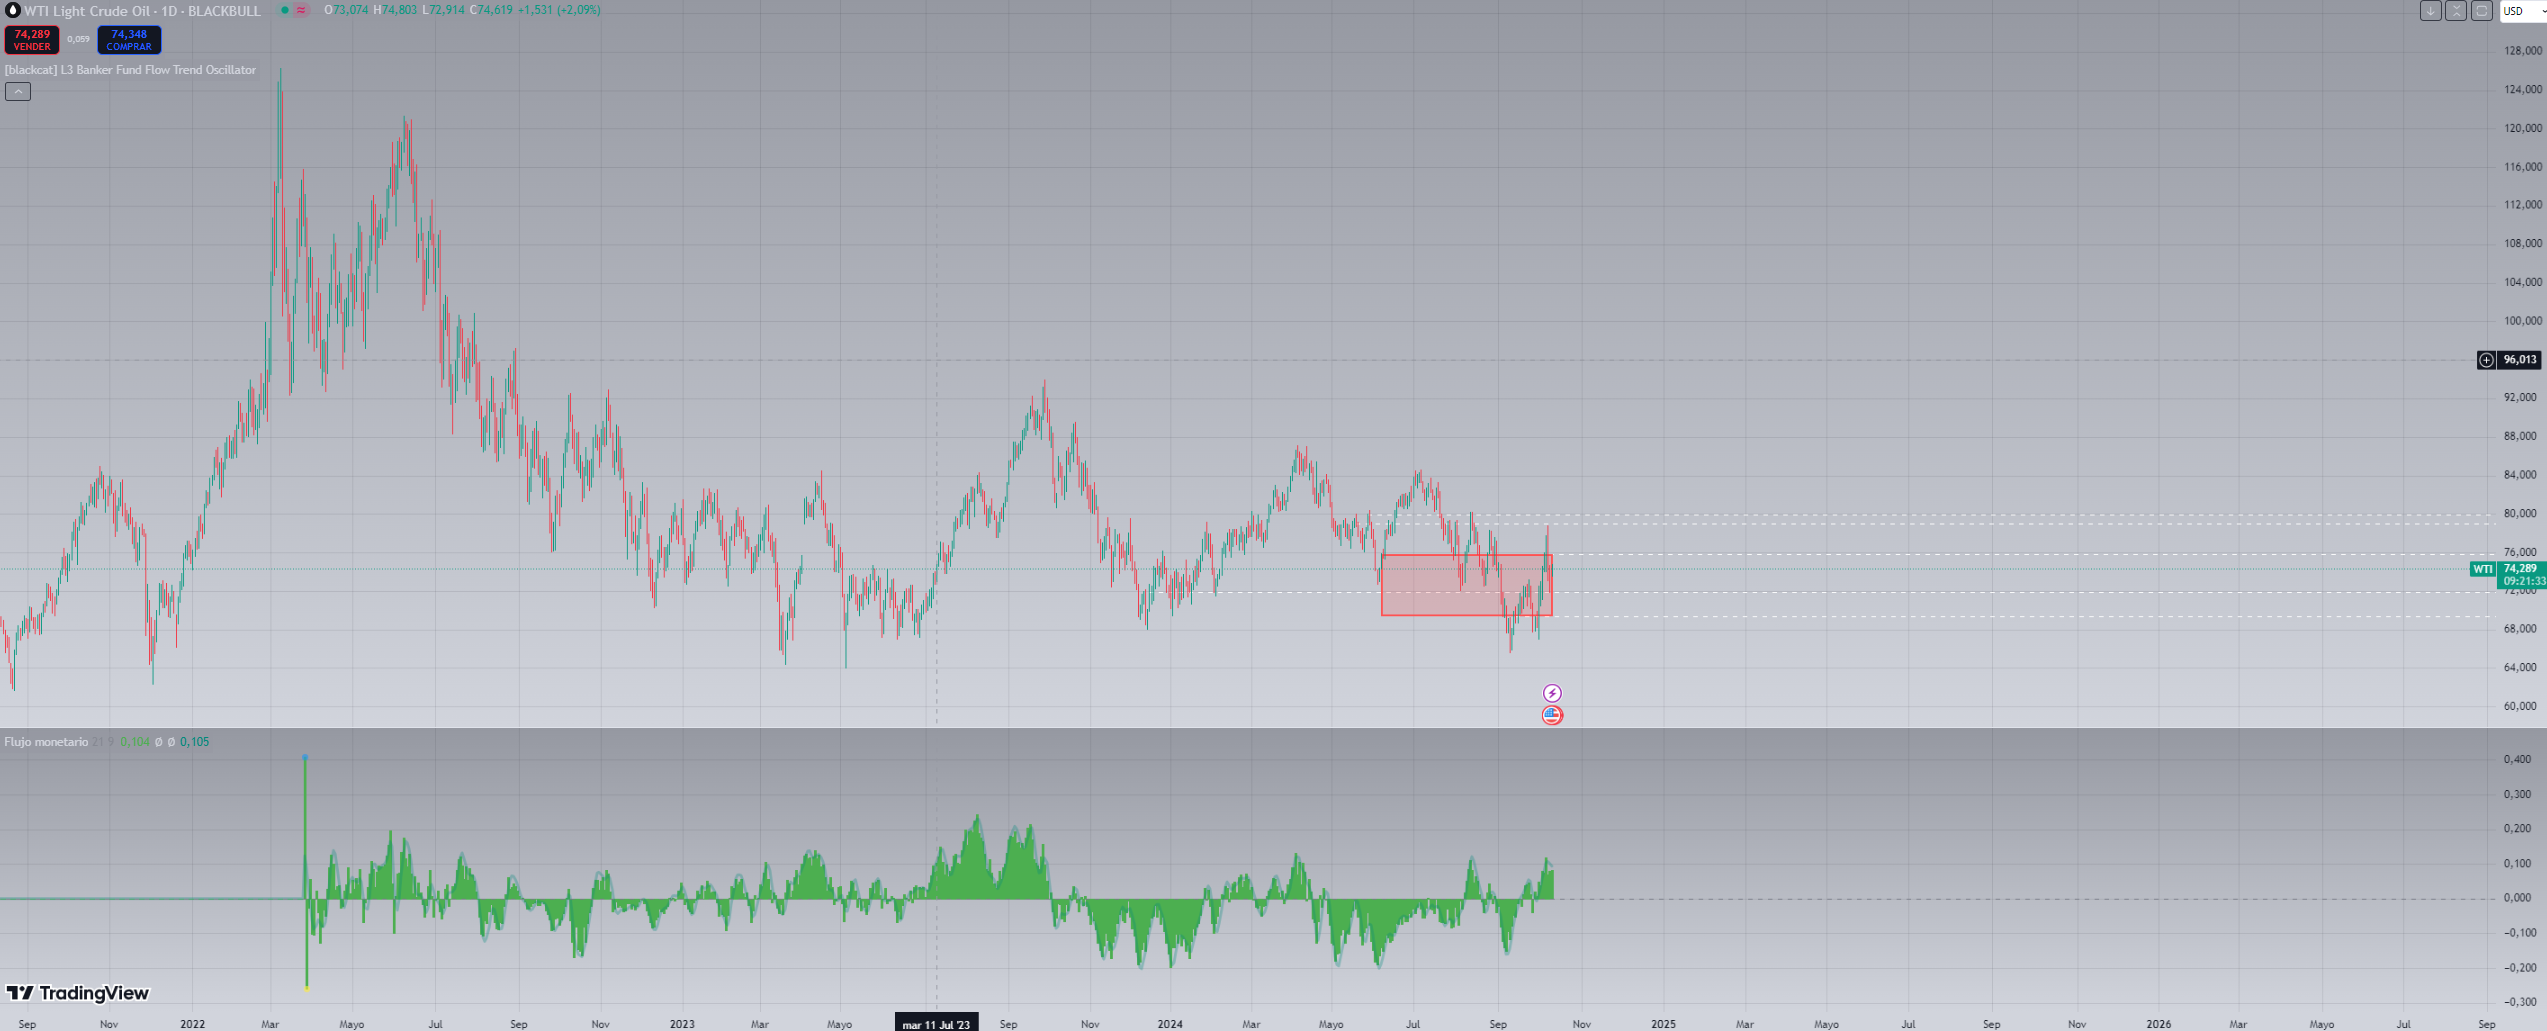
\includegraphics[width=0.8\linewidth]{images/Captura de pantalla 2024-10-10 133834.png} % Sustituir con un gráfico real si se tiene
    \caption{Tendencias del precio del petróleo}
\end{figure}

Esto se debe principalmente a la capacidad de los consumidores de petróleo para cubrirse a través de derivados, lo que ha evitado una subida abrupta del precio. Al mismo tiempo, el incremento en los volúmenes transaccionados en los mercados de derivados desde 2006 ha multiplicado por 15 la liquidez, facilitando una mayor estabilidad en los precios.
\end{frame}

\section{Riesgos Potenciales}
\begin{frame}
\frametitle{Riesgos Potenciales}

Aunque el mercado ha mantenido una prima de guerra baja, existen riesgos importantes que podrían desestabilizar esta situación:

\begin{itemize}
    \item \textbf{Escalamiento del conflicto geopolítico:} Un aumento de las tensiones entre Irán e Israel, con posibles ataques a infraestructuras petroleras clave, podría revertir la actual calma.
    \item \textbf{Inestabilidad en el suministro:} Si el conflicto afecta los estrechos estratégicos como el de Ormuz, el suministro global de petróleo podría verse seriamente comprometido.
    \item \textbf{Políticas de sanciones:} Cualquier cambio en las sanciones a países productores como Venezuela o Irán podría alterar la oferta disponible en el mercado.
\end{itemize}

\end{frame}

\section{Estrategia Recomendada}
\begin{frame}[allowframebreaks] 
\frametitle{Estrategia Recomendada}

Dada la estabilidad actual del mercado petrolero a pesar del riesgo geopolítico, recomendamos una estrategia de inversión diferenciadora basada en patrones de arbitraje intersectorial. Esta estrategia se enfoca en aprovechar las ineficiencias temporales entre sectores relacionados indirectamente con la energía, como:

\begin{itemize}
    \item \textbf{Arbitraje entre sectores de transporte y energía:} Monitorear las discrepancias en la valoración de acciones entre empresas de transporte y proveedores de energía. Una caída en el precio del petróleo suele beneficiar a las empresas de transporte, mientras que las energéticas podrían ser penalizadas. Identificar oportunidades de compra en transporte y venta en energía cuando se observa un desbalance.
    \item \textbf{Indicadores de volatilidad basados en eventos geopolíticos:} Implementar estrategias de cobertura mediante derivados basados en índices de volatilidad (\emph{VIX}) cuando se anticipe un escalamiento del conflicto geopolítico.
    \item \textbf{Rotación sectorial:} Identificar patrones de rotación hacia sectores defensivos como consumo básico y salud, en caso de un incremento en la percepción de riesgo geopolítico o recesión global.
\end{itemize}

\begin{table}[]
    \centering
    \caption{Oportunidades de arbitraje intersectorial}
    \begin{tabular}{|c|c|c|}
    \hline
    Sector        & Relación con precio del petróleo & Oportunidad de inversión \\
    \hline
    Energía       & Negativa                         & Venta \\
    Transporte    & Positiva                         & Compra \\
    Consumo básico & Neutro                          & Compra en tiempos de riesgo \\
    \hline
    \end{tabular}
\end{table}

\end{frame}

\end{document}
